%%% Local Variables:
%%% TeX-master: "slides"
%%% End:

\begingroup
\renewcommand{\insertframenumber}{42}
 \begin{frame}
  \frametitle{Backup}
  \topline
  \vspace{-10px}
  \addtocounter{framenumber}{-1}
 \end{frame}
\endgroup

\begingroup
\renewcommand{\insertframenumber}{43}
 \begin{frame}
  \frametitle{Backup}
  \topline
  \vspace{-10px}
  \addtocounter{framenumber}{-1}
  \begin{block}{Number of grid points vs. accuracy}
    \begin{itemize}
    \item Holds only if $D^2f$ is bounded
    \item Maximal level $n$, maximal dimension $d$
      \vspace{10px}
    \item Number of grid points:
      $$\mathcal{O}(2^{nd}) \ \ \rightarrow \ \ \mathcal{O}(2^{n} \cdot n^{d-1})$$
    \item Error:
      $$\mathcal{O}(2^{-2n}) \ \ \rightarrow \ \ \mathcal{O}(2^{-2n} \cdot n^{d-1})$$
    \end{itemize}
  \end{block}
 \end{frame}
\endgroup

\begingroup
\renewcommand{\insertframenumber}{43}
 \begin{frame}
  \frametitle{Backup}
  \topline
  \vspace{-10px}
  \addtocounter{framenumber}{-1}
  \begin{block}{Implementation}
    \begin{equation*}
      \begin{split}
        \Big(\frac{1}{M} BB^T + \lambda I \Big)\vec{\alpha} = \frac{1}{M}B\vec{y} \\
        \equiv \lambda I\vec{\alpha} + \frac{1}{M}B(B^T)\vec{\alpha} = \frac{1}{M}B\vec{y}
      \end{split}
    \end{equation*}
    \begin{itemize}
    \item $\vec{v}_j = (B^T\vec{\alpha})_j = \hat{f}(x^{(j)})$
    \item $\vec{w} = B\vec{v}$
    \end{itemize}
  \end{block}
 \end{frame}
\endgroup


\begingroup
\renewcommand{\insertframenumber}{43}
 \begin{frame}
  \frametitle{Backup}
  \topline
  \vspace{-10px}
  \addtocounter{framenumber}{-1}
  \begin{block}{Implementation}
    \begin{figure}[!htp]
      \setbeamertemplate{caption}{\raggedright\insertcaption\par}
      \setbeamerfont{caption}{size=\footnotesize}
      \centering
      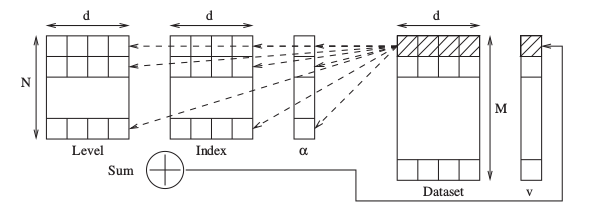
\includegraphics[width=7cm]{images/impl_1}\\
      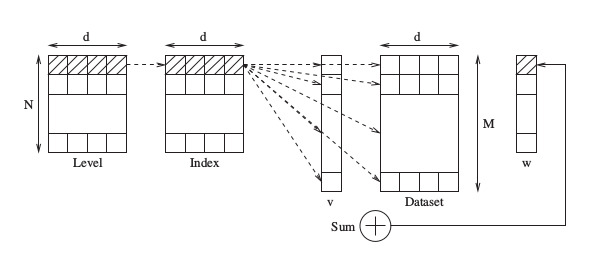
\includegraphics[width=7cm]{images/impl_2}
      \vspace{-12px}
      \caption{}
    \end{figure}
    \vspace{-30px}
    \begin{flushright}
      \tiny{\emph{(Alexander F. Heinecke -- Boosting Scientific Computing Applications\\
through Leveraging
Data Parallel Architectures)}}
    \end{flushright}
  \end{block}
 \end{frame}
\endgroup
